\pdfminorversion=7
\documentclass[conference]{IEEEtran}
\IEEEoverridecommandlockouts

\usepackage[utf8]{inputenc}
\usepackage[T1]{fontenc}
\usepackage[spanish,es-tabla]{babel}
\usepackage{cite}
\usepackage{amsmath,amssymb}
\usepackage{graphicx}
\usepackage{booktabs}
\usepackage{array}
\usepackage{url}
\usepackage{xcolor}
\usepackage{float}

\graphicspath{{../figuras/}}
\setlength{\textfloatsep}{7pt}
\setlength{\floatsep}{6pt}
\setlength{\intextsep}{6pt}

\begin{document}

\title{Diseño e implementación de una tarjeta de acondicionamiento de señales para sensores de torque y temperatura en un motor de inducción}

\author{\IEEEauthorblockN{Kenneth Daniel Vizcaíno Jiménez}
\IEEEauthorblockA{\textit{Escuela de Ingeniería Eléctrica}\\
\textit{Universidad de Costa Rica}\\
San José, Costa Rica\\
kenneth.vizcaino@ucr.ac.cr}}

\maketitle

\begin{abstract}
Este reporte documenta el diseño de una tarjeta de acondicionamiento para sensores de torque y temperatura instalados en un motor de inducción del LabCES. El propósito del proyecto es adaptar las señales de un PT100 y una celda SM-50 para facilitar su adquisición y monitoreo en el banco de pruebas. El trabajo partió de modelos eléctricos, se verificó en LTspice y se trasladó a KiCad para obtener una PCB lista para fabricación. El PT100 se excitó con baja corriente para reducir autocalentamiento y el SM-50 se amplificó hasta $\pm4.39$ V, dentro del rango de $\pm5$ V de la B-Box. El resultado actual incluye simulaciones, esquemático, PCB, validación ERC/DRC y paquete Gerber; la prueba con prototipo físico queda como cierre posterior.
\end{abstract}

\begin{IEEEkeywords}
PT100, SM-50, motor de inducción, puente Wheatstone, INA826, LTspice, KiCad, acondicionamiento de señal, B-Box.
\end{IEEEkeywords}

\section{Introducción}

El proyecto nace de una necesidad práctica: medir temperatura y torque en un motor trifásico de inducción sin depender de señales crudas, pequeñas o vulnerables al ruido. En el banco del LabCES, estas variables apoyan el análisis del desempeño del motor, por lo que la PCB se planteó como una etapa intermedia entre los sensores y la interfaz de adquisición. El objetivo general propuesto fue diseñar e implementar una tarjeta de circuito impreso que acondicione y adapte esas señales para facilitar su adquisición y monitoreo.

La propuesta se organizó alrededor de cuatro objetivos específicos: comprender el diseño de PCB aplicado al acondicionamiento de señales con KiCad; verificar los sensores mediante pruebas o antecedentes reales disponibles; diseñar la PCB del circuito de acondicionamiento; e implementar y probar el prototipo dentro del sistema del motor. Como entregables se propusieron repositorio Git, diseño completo, prototipo físico, manual de instalación y uso, y sistema probado en el banco del LabCES.

Este documento reporta el estado técnico alcanzado: diseño electrónico completo, simulación, justificación de valores, diseño en KiCad y paquete de fabricación. Los entregables que dependen de una PCB ensamblada se presentan como pendientes de validación experimental, no como resultados ya ejecutados.

\section{Criterios de diseño}

La ruta de señal se definió siguiendo la arquitectura recomendada para sensores resistivos: excitación estable, transductor, amplificación, filtrado y adquisición. Analog Devices resume esta idea para sensores de fuerza y temperatura, indicando que las señales de puentes y RTD requieren una cadena que cuide excitación, ganancia, ruido, rechazo de modo común y ancho de banda antes de llegar al ADC \cite{adi_paths}. Por eso la tarjeta no se diseñó como una suma de bloques sueltos, sino como dos rutas completas: PT100--referencia--amplificación--filtro--B-Box y SM-50--excitación--INA--filtro--B-Box.

La restricción de adquisición más importante fue el rango de entrada de la B-Box. La documentación de imperix reporta entradas analógicas diferenciales de $\pm5$ V y alimentación de sensores de $\pm15$ V limitada a 100 mA \cite{imperix}. Con ese dato, el diseño no se planteó para llegar exactamente a $\pm5$ V, sino para quedar cerca y conservar margen frente a tolerancias, offset y calibración.

Para el PT100 se usó la relación de resistencia de un RTD de platino según IEC 60751: a 100 $^\circ$C se espera cerca de 138.5 $\Omega$ \cite{bipm}. La excitación se fijó en 0.5 mA con una referencia REF3012 de 1.25 V \cite{ref30} y una resistencia de 2.49 k$\Omega$, un valor moderado que produce señal medible sin calentar el sensor más de lo necesario. Los cálculos completos se dejaron en el Anexo A.

Para el SM-50 se partió de su naturaleza de puente de galgas: 350 $\Omega$, salida nominal de 3 mV/V y uso en tensión/compresión \cite{interface}. Con 10 V de excitación se obtienen 30 mV diferenciales a escala completa, por lo que se usó el INA826 para llevar la señal a $\pm4.39$ V con $R_G=340~\Omega$ \cite{ina826}. Esta arquitectura coincide con notas de TI y Analog Devices sobre puentes Wheatstone: excitar el puente, medir diferencialmente con rechazo de modo común y filtrar antes de adquirir \cite{sloa034}, \cite{sboa247}, \cite{an43}. También se evitó subir la ganancia sin criterio, porque el ruido y la deriva entran al mismo frente analógico \cite{an96}.

\subsection{Justificación numérica de los valores}

En el canal PT100, Analog Devices y Texas Instruments muestran que una medición RTD se suele resolver con corriente de excitación, referencia estable, ganancia y ADC de precisión \cite{adi_rtd}, \cite{ti_rtd}. El valor de 0.5 mA se defendió por sensibilidad suficiente, autocalentamiento bajo y compatibilidad con la B-Box. El span amplificado fue de aproximadamente 0.970 V entre 0 y 100 $^\circ$C; el detalle numérico está en el Anexo A.

En el canal SM-50, la hoja del sensor fija los tres datos de partida: 3.0 mV/V, puente de 350 $\Omega$ y excitación máxima de 15 VDC \cite{interface}. Se eligió 10 V porque genera 30 mV diferenciales a escala completa, mantiene la corriente del puente en 28.6 mA y evita subir la disipación del sensor al caso de 15 V. La ganancia necesaria para llevar esa señal a un rango cercano a $\pm4.4$ V coincide con el INA826 usando $R_G=340~\Omega$. Esta forma de escoger la ganancia sigue el criterio de diseños de puente ya publicados: primero se define el swing de salida permitido por el ADC y luego se calcula la ganancia desde el diferencial máximo esperado \cite{sboa247}.

Los filtros también se escogieron con una idea de ruta de señal, no solo por costumbre. ADI recomienda limitar el ancho de banda cuando el transductor es lento y sensible al ruido \cite{adi_paths}. Por eso se usaron filtros RC de salida: para PT100 se dejó un corte cercano a 159 Hz y para SM-50 uno cercano a 482 Hz. Ambos valores son suficientemente altos para no borrar la dinámica esperada del banco, pero reducen ruido antes de la adquisición. Las fórmulas de corte y la tabla de valores quedaron concentradas en el Anexo A.

\subsection{Diseño por etapas o ciudades}

El diseño no se hizo como un esquemático grande de una sola vez. Se trabajó por etapas, llamadas en la bitácora ``ciudades'', para separar las señales de milivoltios de las zonas de alimentación, protección y conectores \cite{bitacora}. Esta decisión reduce el riesgo de acoplar ruido en rutas sensibles como el SM-50, que entrega hasta 30 mV antes de amplificar.

Las ciudades usadas fueron: entrada y excitación del SM-50; acondicionamiento de torque con INA, ganancia y filtrado; entrada PT100 con fuente de corriente y líneas de sense; acondicionamiento de temperatura con offset, ganancia y filtrado; alimentación/protección desde B-Box; y salidas RJ45 hacia la B-Box. Esta forma de diseño permitió que cada ciudad tuviera una función clara: primero proteger y excitar el sensor, luego amplificar una señal pequeña, después filtrar, ajustar y finalmente entregar una señal robusta al sistema de adquisición.

\subsection{Selección de componentes y filtros}

Los valores de resistencias y capacitores se eligieron según su papel en la ruta de señal. En el PT100, $R_{\text{SET}}=2.49~\text{k}\Omega$ produce 0.5 mA con la referencia de 1.25 V; por eso se usó tolerancia baja. Las resistencias de entrada de 49.9 $\Omega$ y capacitores de 10 nF no buscan ganancia, sino limitar picos rápidos y atenuar ruido de alta frecuencia antes del INA sin volver lenta la medición.

El filtro principal se dejó como pasabajo RC de primer orden porque temperatura y torque son lentos frente al ruido eléctrico del banco. El corte de 159 Hz del PT100 no deforma la dinámica térmica, y el de 482 Hz del SM-50 conserva más banda para cambios de carga. Los 100 nF de desacoplo cerca de referencias, operacionales, INA y reguladores se usaron como reserva local de carga.

El trimmer multivuelta Bourns 3296W de 1 k$\Omega$ se incluyó como ajuste fino de laboratorio. No se usó para ``adivinar'' la ganancia, ya calculada por $R_G$, sino para corregir tolerancias, offset del puente, ruido del banco y dispersión de montaje. Al ser multivuelta permite ajustes pequeños y repetibles \cite{bourns3296}, de modo que RV1/RV2 dan margen de calibración sin rediseñar la PCB.

\section{Simulación en LTspice}

Las simulaciones se separaron por canal para depurar cada sensor sin mezclar errores. Primero se trabajó el PT100, luego el SM-50, y después se exportaron los barridos numéricos para regenerar las gráficas. Este flujo deja el resultado repetible si cambia un parámetro y mantiene el reporte centrado en el método seguido.

En el PT100, el barrido de 0 a 100 $^\circ$C confirmó que la resistencia sube de 100 $\Omega$ a 138.5 $\Omega$ y que la salida acondicionada aumenta de 2.33 V a 3.22 V. Esta salida absoluta incluye el punto de operación del circuito; lo importante es que el cambio de temperatura produce una variación clara, continua y dentro del rango de lectura.

En el SM-50, la simulación bipolar barrió de -50 lb a +50 lb. La tensión diferencial del puente llegó a $\pm30$ mV y, con $R_G=340~\Omega$, la salida del INA826 llegó a $\pm4.3888$ V, dejando alrededor de 0.61 V de margen antes de $\pm5$ V. Así se comprobó que la ganancia calculada era coherente con la interfaz de adquisición.

Además, los resultados se compararon con una investigación previa del banco LabCES con datos reales de sensores \cite{labces_prev}. En el PT100, las resistencias medidas a 0, 20, 50 y 100 $^\circ$C fueron aproximadamente 100.000, 107.793, 119.395 y 138.500 $\Omega$, muy cercanas al modelo usado en LTspice. En el SM-50, los datos previos mostraban offset y comportamiento no suficientemente limpio para tomarlos como calibración final; por eso se usaron como antecedente del problema. La calibración real debe hacerse con la PCB fabricada y cargas conocidas.

Para no saturar el cuerpo del reporte, las gráficas de simulación se colocaron en el Anexo B. En el texto principal se conservan únicamente los resultados que justifican las decisiones de diseño.

\section{Implementación en KiCad}

Después de validar los rangos en LTspice, el circuito se trasladó a KiCad. La PCB se organizó por bloques: entrada PT100, entrada SM-50, referencia/excitación, amplificación, filtrado, protección y salida hacia la B-Box. Esta separación ayudó a mantener trazabilidad entre cálculo, simulación y esquemático.

La selección de componentes siguió la función de cada etapa. El REF3012 entregó la referencia de 1.25 V para fijar la corriente del PT100 \cite{ref30}; el OPA2188 se usó donde convenía baja deriva y bajo offset \cite{opa2188}; el TPS7A4901 se seleccionó como regulador positivo de bajo ruido para la excitación del puente \cite{tps7a49}; y el INA826 se mantuvo por su ganancia ajustable y rechazo de modo común \cite{ina826}.

La parte mecánica también se justificó. Se usaron librerías locales de símbolos, footprints y modelos 3D; los integrados quedaron con encapsulados específicos; el TPS7A4901DGNT mantuvo su footprint DGN-8 con pad térmico; y los sensores se separaron en bornera de 3 pines para PT100 y de 4 pines para SM-50. La auditoría de footprints evitó mezclar modelos 3D con land patterns no verificados.

\subsection{Grosores y anchos de pista}

El stackup del proyecto se dejó como tarjeta de 1.6 mm con cobre externo de 35 $\mu$m, equivalente al cobre comercial típico de 1 oz. En la revisión del layout y del paquete Gerber se confirmaron pistas rutadas de 0.20, 0.25, 0.30, 0.40, 0.50, 0.60 y 0.80 mm. Los anchos principales del diseño sí están entre 0.25 y 0.60 mm; el valor de 0.20 mm aparece solo en dos segmentos puntuales y el de 0.80 mm en diez segmentos robustos de alimentación y retorno. La documentación oficial de KiCad indica que estas reglas de diseño gobiernan el ruteo, la verificación DRC y los anchos disponibles durante el trazado \cite{kicad_pcbnew}.

La decisión no fue solo por espacio. El criterio eléctrico se revisó con el modelo IPC-2221 para pistas externas, usando 1 oz de cobre y 10 $^\circ$C de aumento térmico como caso conservador \cite{digikey_trace}. Aun una pista de 0.25 mm soporta del orden de 0.88 A bajo ese criterio, muy por encima de las corrientes reales del diseño: 0.5 mA en el PT100, 28.6 mA en el puente SM-50 y 100 mA como límite de alimentación de sensores de la B-Box. Por eso las pistas de 0.50, 0.60 y 0.80 mm no se eligieron porque la corriente lo exigiera al límite, sino para reducir caída de tensión, mejorar robustez en conectores y separar físicamente potencia/retorno de las señales de milivoltios. La tabla completa de anchos y márgenes queda en el Anexo A.

Las vistas del diagrama funcional y de la PCB final se movieron al Anexo B para dejar el desarrollo principal más limpio.

\section{Validación y cumplimiento frente a la propuesta}

El primer objetivo se cubrió al aplicar fundamentos de PCB, ruteo por etapas, selección de anchos de pista, revisión de footprints y uso de KiCad. El segundo objetivo se atendió con simulaciones LTspice de los canales PT100 y SM-50, y con la comparación contra una investigación previa del banco que contenía datos reales de sensores. La verificación definitiva con la PCB final debe hacerse después de fabricar el prototipo.

El tercer objetivo se completó con el esquemático, layout, librerías locales, validaciones y paquete de fabricación. El cuarto objetivo, implementar y probar el prototipo en el sistema de medición, queda como cierre experimental pendiente porque la tarjeta aún no se ha fabricado ni ensamblado. En entregables, ya se cuenta con repositorio técnico, diseño completo, cálculos, simulaciones, validaciones ERC/DRC y paquete Gerber; quedan por completar el prototipo ensamblado, el manual final y la prueba integrada en el banco del LabCES.

La validación de cierre reportó 0 errores ERC, 0 advertencias ERC, 0 violaciones DRC, 0 pads desconectados y 0 errores de footprint. Además, el paquete de fabricación incluye las capas de cobre, máscara, pasta, serigrafía, contorno, descripción del trabajo, taladros y mapa de perforaciones. Esto no reemplaza una prueba eléctrica en laboratorio, pero sí confirma que el diseño digital quedó coherente y fabricable.

\section{Conclusiones}

El proyecto logró convertir una necesidad de medición del banco LabCES en una PCB trazable, simulada y preparada para fabricación. En el PT100, la corriente de 0.5 mA se escogió porque da sensibilidad suficiente sin castigar el sensor con autocalentamiento. En el SM-50, la excitación de 10 V y $R_G=340~\Omega$ permiten llevar una señal de $\pm30$ mV hasta $\pm4.39$ V, rango cómodo para la B-Box. Frente a la propuesta original, el diseño electrónico y la documentación técnica quedan cubiertos; la calibración real, el manual final y la prueba integrada deben cerrarse con el prototipo físico, usando resistencias patrón y cargas conocidas.

\clearpage
\section*{Anexo A: Cálculos y tablas de respaldo}

\subsection*{A.1 Canal PT100}

El modelo usado para el PT100 en el rango positivo fue
\begin{equation}
R(T)=R_0(1+AT+BT^2),
\end{equation}
donde $R_0=100~\Omega$, $A=3.9083\times10^{-3}$ y $B=-5.775\times10^{-7}$ \cite{bipm}. Con esto, $R(100^\circ\text{C})\approx138.5~\Omega$.

La corriente de excitación se calculó a partir de la referencia y la resistencia de ajuste:
\begin{equation}
I_{\text{PT100}}=\frac{1.25~\text{V}}{2.49~\text{k}\Omega}=0.502~\text{mA}.
\end{equation}
El span crudo entre 0 y 100 $^\circ$C queda como
\begin{equation}
\Delta V_{\text{PT100}}=0.5~\text{mA}(138.5-100)\Omega=19.25~\text{mV}.
\end{equation}
Con $R_G=1~\text{k}\Omega$ en el INA826, $G=50.40$ V/V, de modo que el span amplificado es cercano a 0.970 V. Para una B-Box de 16 bits sobre 10 V de span, el LSB ideal es 152.6 $\mu$V, equivalente a una resolución eléctrica estimada de 0.0157 $^\circ$C/LSB. El autocalentamiento también queda bajo: con $\Delta T=I^2R/E$ y $E=2.5$ mW/$^\circ$C, la potencia máxima en el PT100 es 34.6 $\mu$W y el error térmico calculado es cercano a 0.014 $^\circ$C \cite{ti_rtd}.

\subsection*{A.2 Canal SM-50}

La salida de escala completa del puente, usando 10 V de excitación, fue
\begin{equation}
V_{\text{diff,FS}}=3~\text{mV/V}\cdot10~\text{V}=30~\text{mV}.
\end{equation}
La corriente y potencia del puente se estimaron como
\begin{equation}
I_{\text{puente}}=\frac{10~\text{V}}{350~\Omega}=28.6~\text{mA},
\end{equation}
\begin{equation}
P_{\text{puente}}=\frac{(10~\text{V})^2}{350~\Omega}=286~\text{mW}.
\end{equation}
Para llevar 30 mV a aproximadamente 4.39 V se necesita una ganancia de 146.3 V/V. Con el INA826:
\begin{equation}
G=1+\frac{49.4~\text{k}\Omega}{R_G},
\end{equation}
y usando $R_G=340~\Omega$, se obtiene $G=146.29$ V/V.

\subsection*{A.3 Filtros}

Los filtros de salida se calcularon como pasabajos RC de primer orden:
\begin{equation}
f_c=\frac{1}{2\pi RC}.
\end{equation}
Para PT100, $R=10~\text{k}\Omega$ y $C=100~\text{nF}$ dan $f_c\approx159$ Hz. Para SM-50, $R=10~\text{k}\Omega$ y $C=33~\text{nF}$ dan $f_c\approx482$ Hz.

\begin{table}[H]
\caption{Resumen de valores principales usados en el diseño}
\label{tab:valores}
\centering
\scriptsize
\begin{tabular}{@{}p{0.18\linewidth} p{0.31\linewidth} p{0.37\linewidth}@{}}
\toprule
Bloque & Valor o resultado & Justificación \\
\midrule
B-Box & $\pm5$ V, 16 bits & Define margen y resolución de salida \cite{imperix}. \\
PT100 & $R(100^\circ\text{C})\approx138.5~\Omega$ & Rango térmico de referencia \cite{bipm}. \\
PT100 & $I_{\text{exc}}=0.502$ mA & Señal útil con bajo autocalentamiento \cite{ti_rtd}. \\
PT100 & $G=50.40$ V/V; span 0.970 V & Compatible con adquisición sin saturar. \\
SM-50 & 10 V de excitación; 30 mV FS & Dato nominal del sensor \cite{interface}. \\
SM-50 & $G=146.29$ V/V; salida $\pm4.39$ V & Escala la señal al rango de la B-Box. \\
Filtros & 159 Hz PT100; 482 Hz SM-50 & Atenúa ruido sin eliminar dinámica útil \cite{adi_paths}. \\
\bottomrule
\end{tabular}
\end{table}

\subsection*{A.4 Anchos de pista de la PCB}

Para revisar el margen térmico de las pistas se usó la relación IPC-2221 para pistas externas:
\begin{equation}
I=k(\Delta T)^bA^c,
\end{equation}
donde para capas externas $k=0.048$, $b=0.44$ y $c=0.725$ \cite{digikey_trace}, \cite{cirexx_trace}. El cálculo se hizo con cobre de 1 oz, $\Delta T=10^\circ$C y pistas externas. Estos resultados son estimados, pero sirven para demostrar que el diseño no está cerca de un límite térmico.

\begin{table}[H]
\caption{Anchos de pista confirmados en el diseño y margen estimado de corriente}
\label{tab:pistas}
\centering
\tiny
\setlength{\tabcolsep}{2pt}
\begin{tabular}{@{}p{0.14\linewidth} p{0.30\linewidth} p{0.17\linewidth} p{0.22\linewidth}@{}}
\toprule
Ancho & Uso en la PCB & $I_{\max}$ est. & Caída, 100 mA/50 mm \\
\midrule
0.20 mm & Segmentos puntuales confirmados & 0.74 A & 12.31 mV \\
0.25 mm & Señales analógicas; ancho dominante & 0.88 A & 9.85 mV \\
0.30 mm & Ajustes y salidas locales & 1.00 A & 8.21 mV \\
0.40 mm & Referencias y tramos intermedios & 1.23 A & 6.16 mV \\
0.50 mm & Rieles protegidos y conectores & 1.45 A & 4.93 mV \\
0.60 mm & Alimentación con margen extra & 1.65 A & 4.10 mV \\
0.80 mm & Retorno/alimentación puntual & 2.03 A & 3.08 mV \\
\bottomrule
\end{tabular}
\end{table}

\begin{figure*}[t]
\centering
{\Large\scshape Anexo B: Figuras de simulación y KiCad\par}
\vspace{4pt}
\begin{minipage}{0.49\linewidth}
\centering
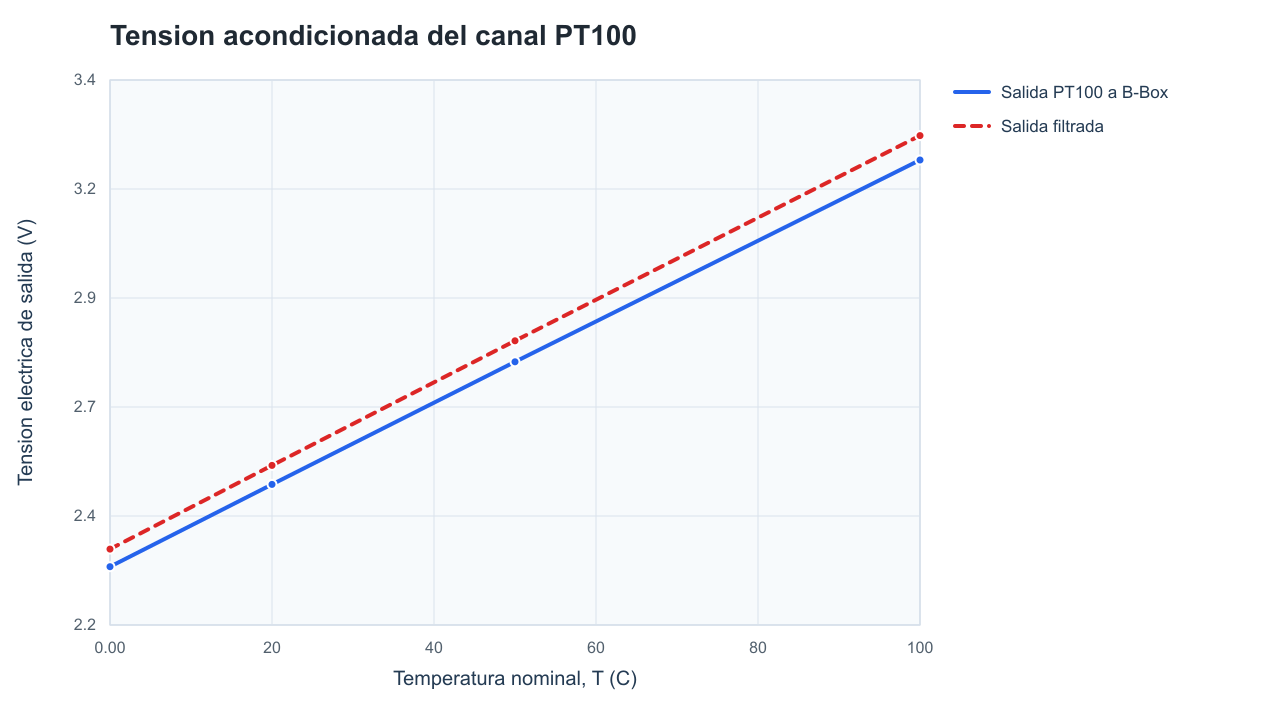
\includegraphics[width=\linewidth]{respuesta_pt100.png}
\end{minipage}
\hfill
\begin{minipage}{0.49\linewidth}
\centering
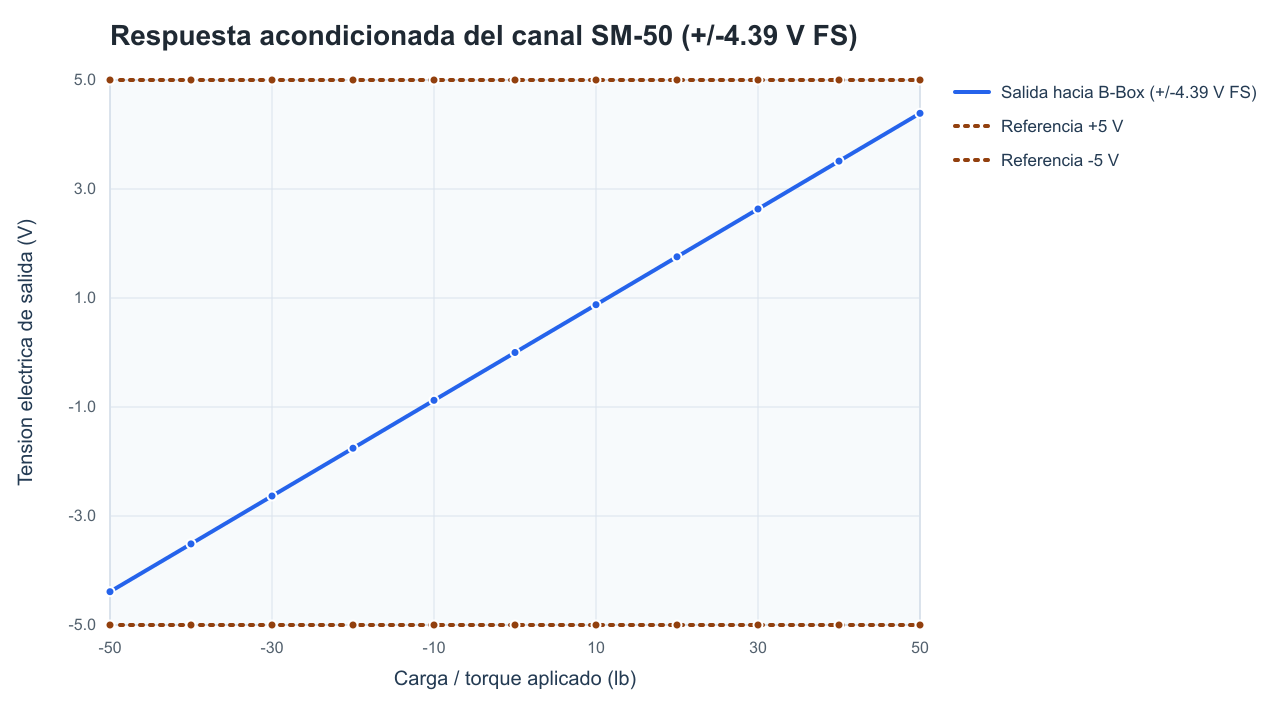
\includegraphics[width=\linewidth]{respuesta_sm50_bipolar.png}
\end{minipage}
\caption{Resultados de simulación usados para validar los rangos de salida. Izquierda: respuesta del canal PT100. Derecha: salida bipolar del SM-50 dentro de $\pm5$ V.}
\label{fig:sim}
\end{figure*}

\begin{figure*}[t]
\centering
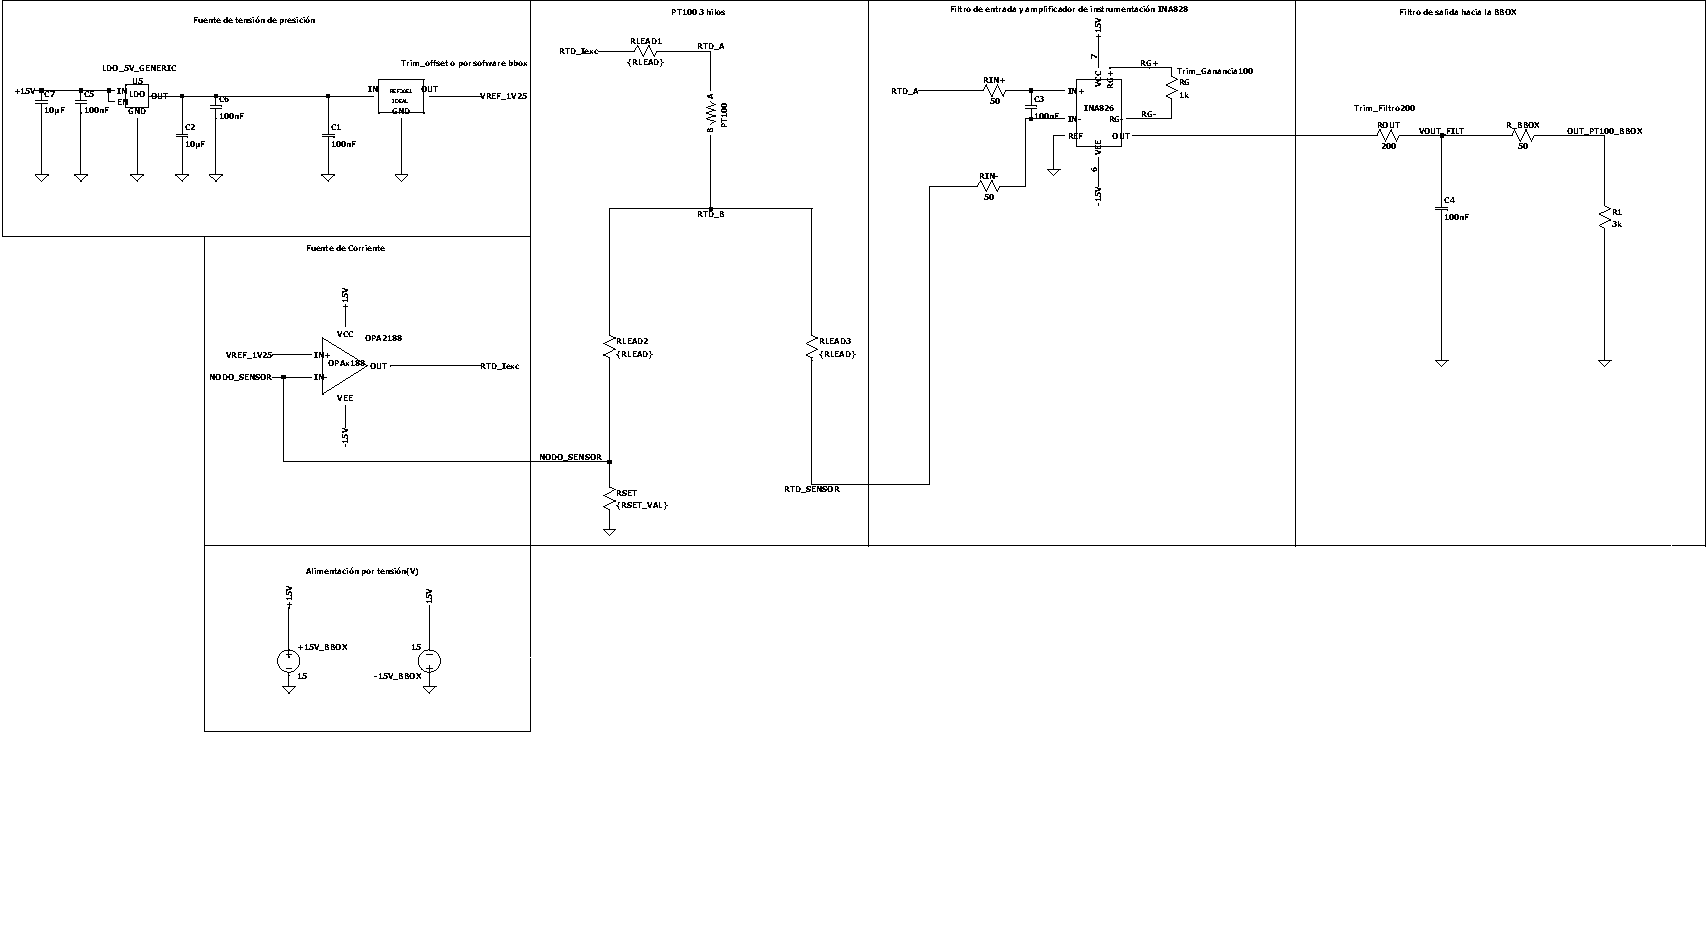
\includegraphics[width=0.95\textwidth]{ltspice_pt100_esquematico_recortado.pdf}
\caption{Esquemático de simulación en LTspice para el canal PT100.}
\label{fig:ltspice_sch}
\end{figure*}

\begin{figure*}[t]
\centering
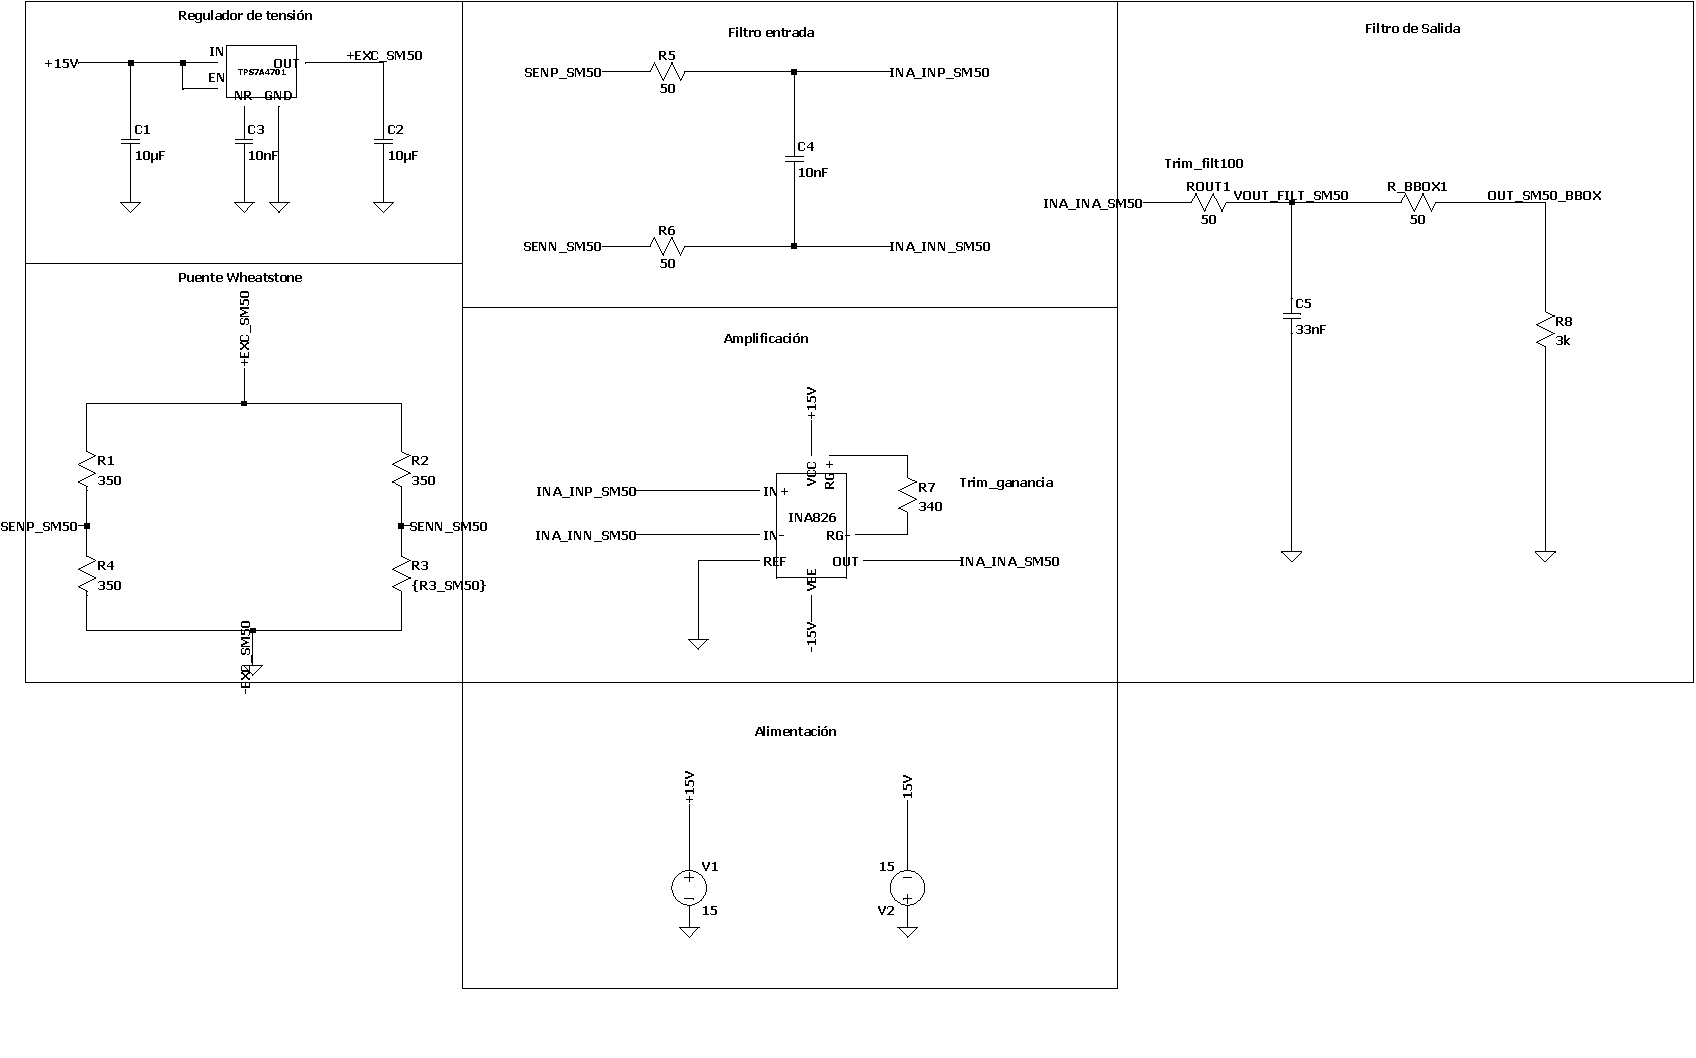
\includegraphics[width=0.95\textwidth]{ltspice_sm50_esquematico_recortado.pdf}
\caption{Esquemático de simulación en LTspice para el canal SM-50.}
\label{fig:ltspice_sm50_sch}
\end{figure*}

\begin{figure*}[t]
\centering
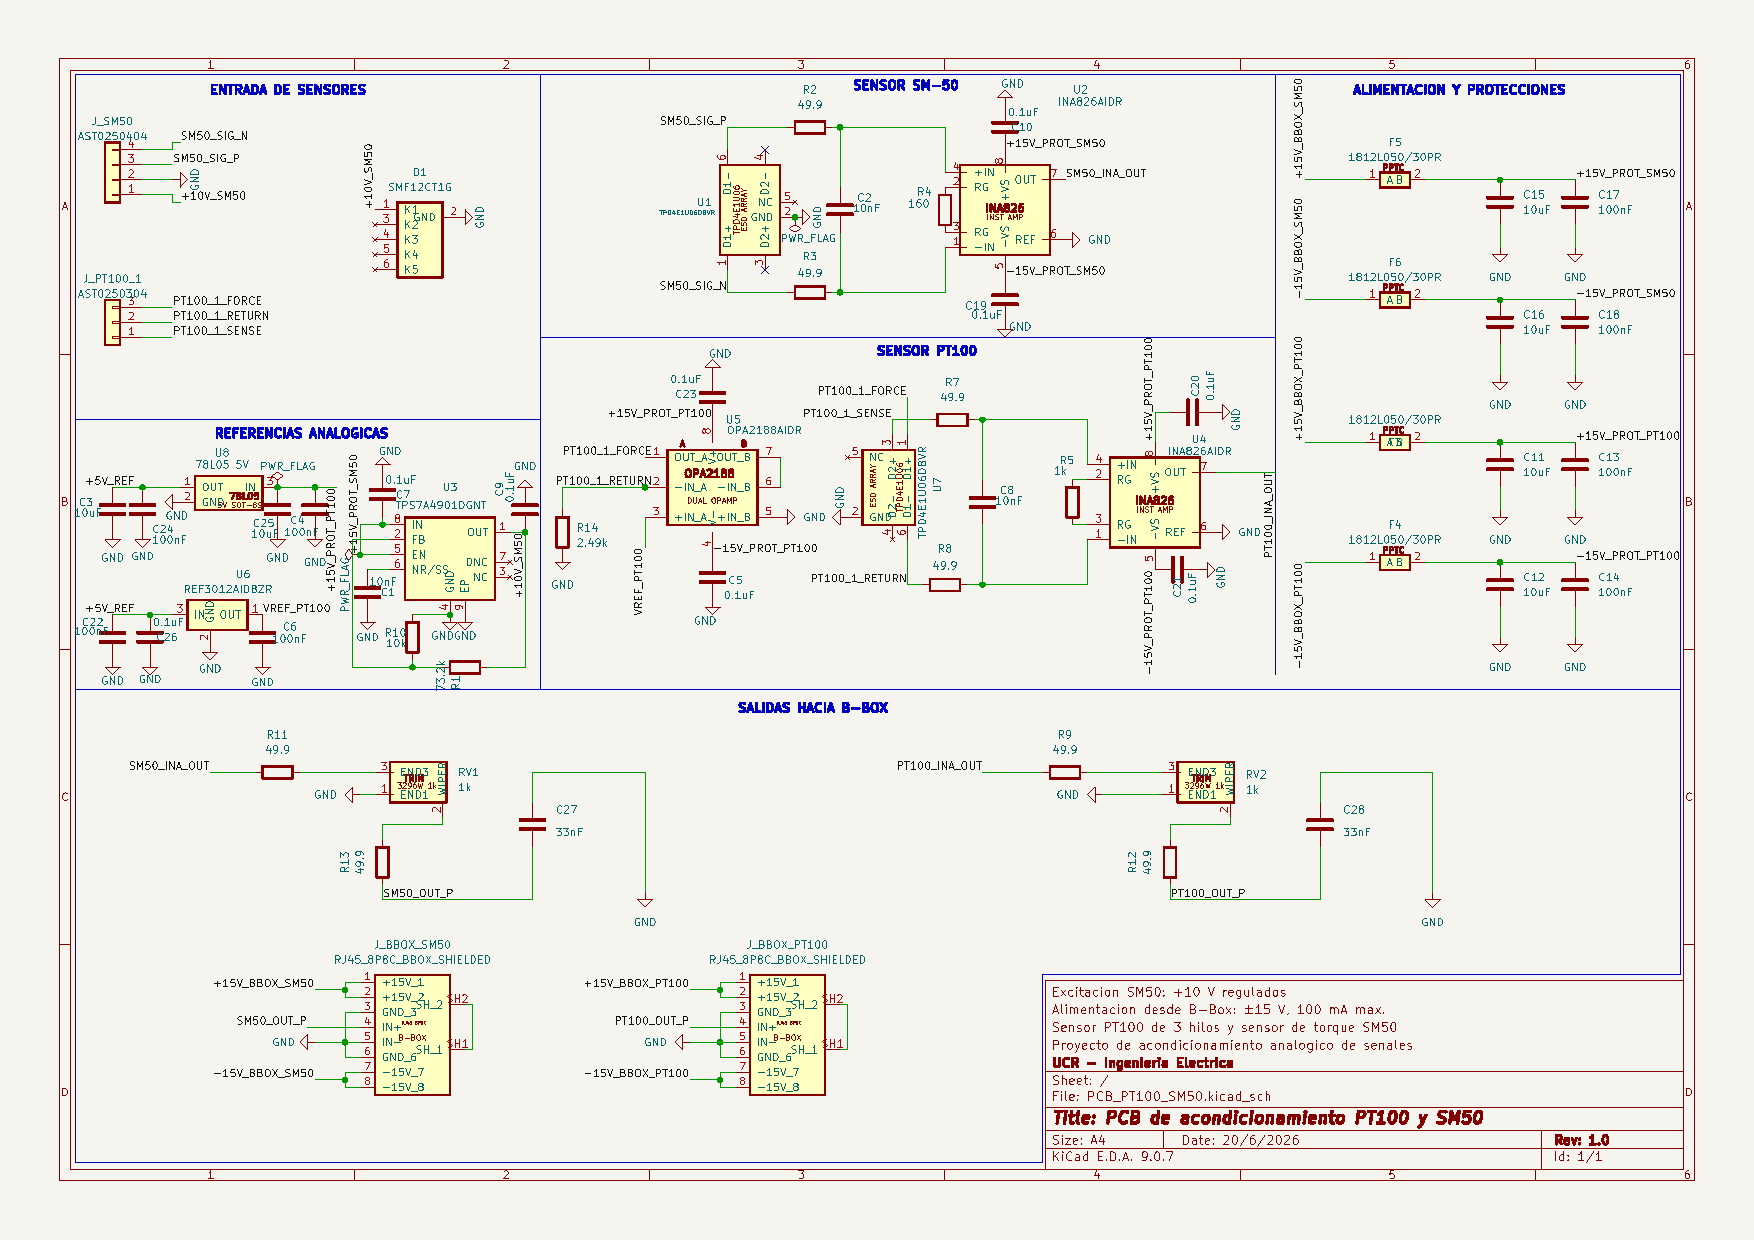
\includegraphics[width=0.95\textwidth]{kicad_esquematico.pdf}
\caption{Esquemático principal de la tarjeta de acondicionamiento implementado en KiCad.}
\label{fig:kicad_sch}
\end{figure*}

\begin{figure*}[t]
\centering
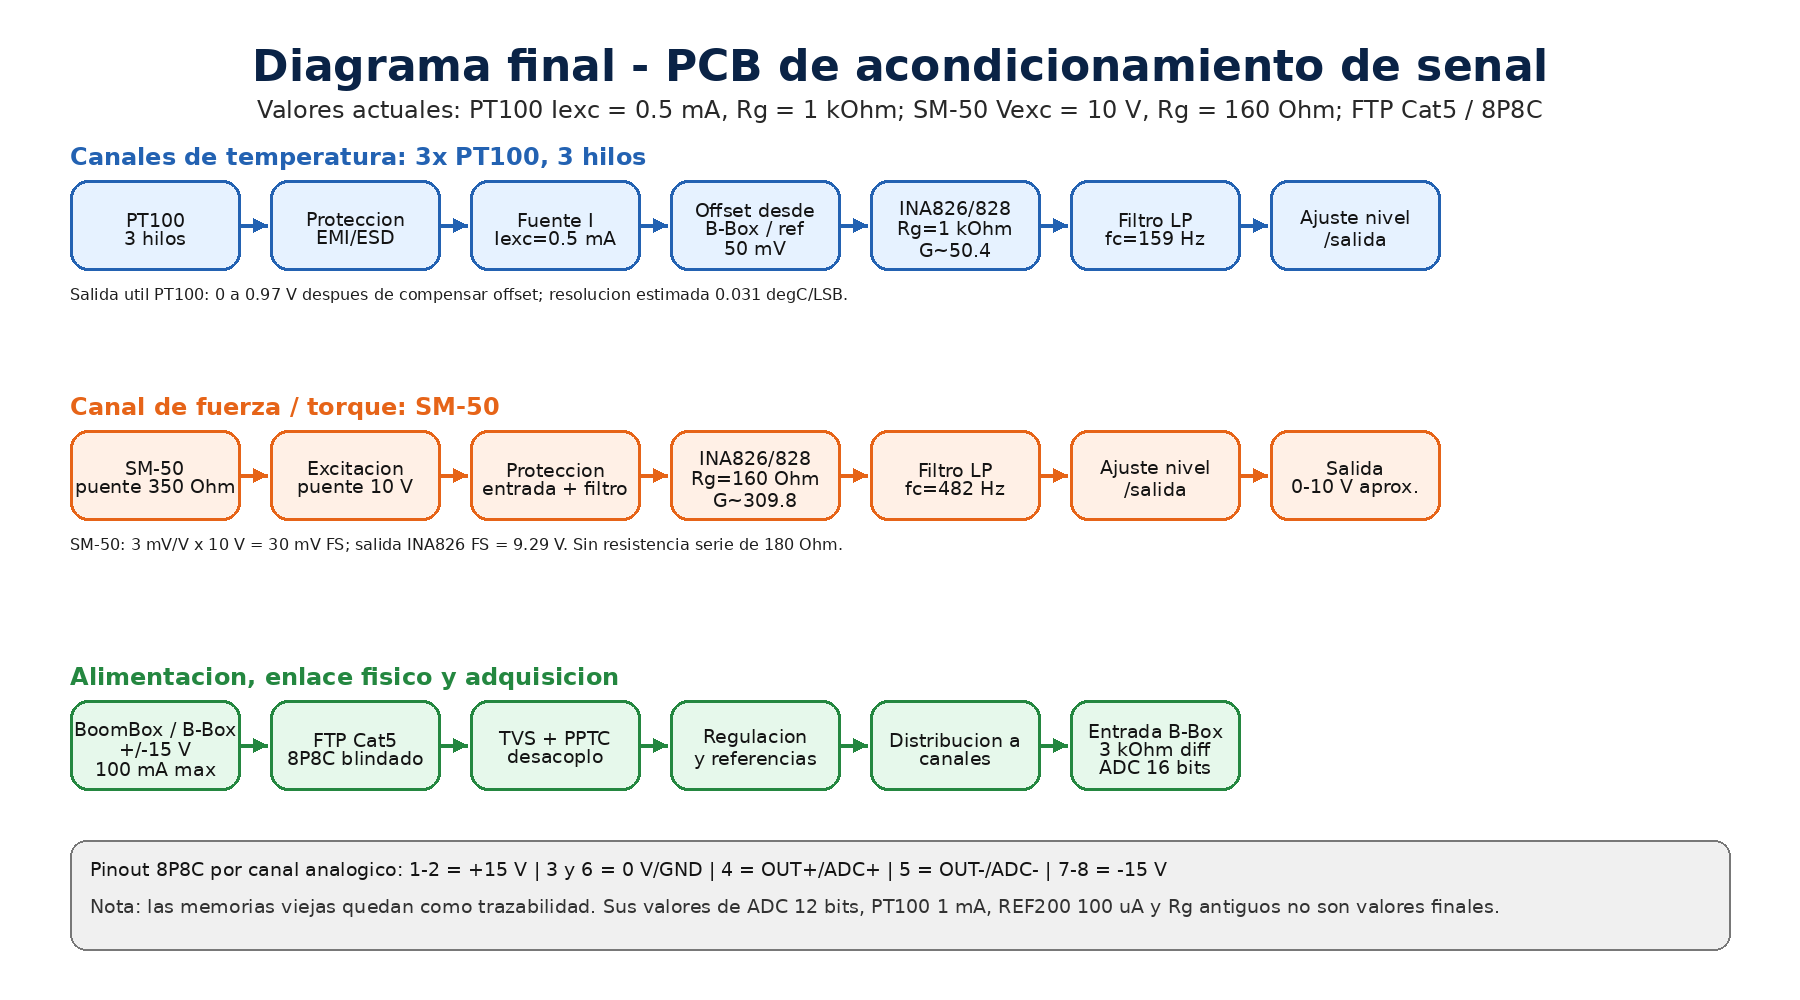
\includegraphics[width=0.95\textwidth]{diagrama_bloques_valores_actuales.png}
\caption{Diagrama funcional del acondicionamiento, con los valores finales usados para PT100, SM-50 e interfaz B-Box.}
\label{fig:bloques}
\end{figure*}

\begin{figure*}[t]
\centering
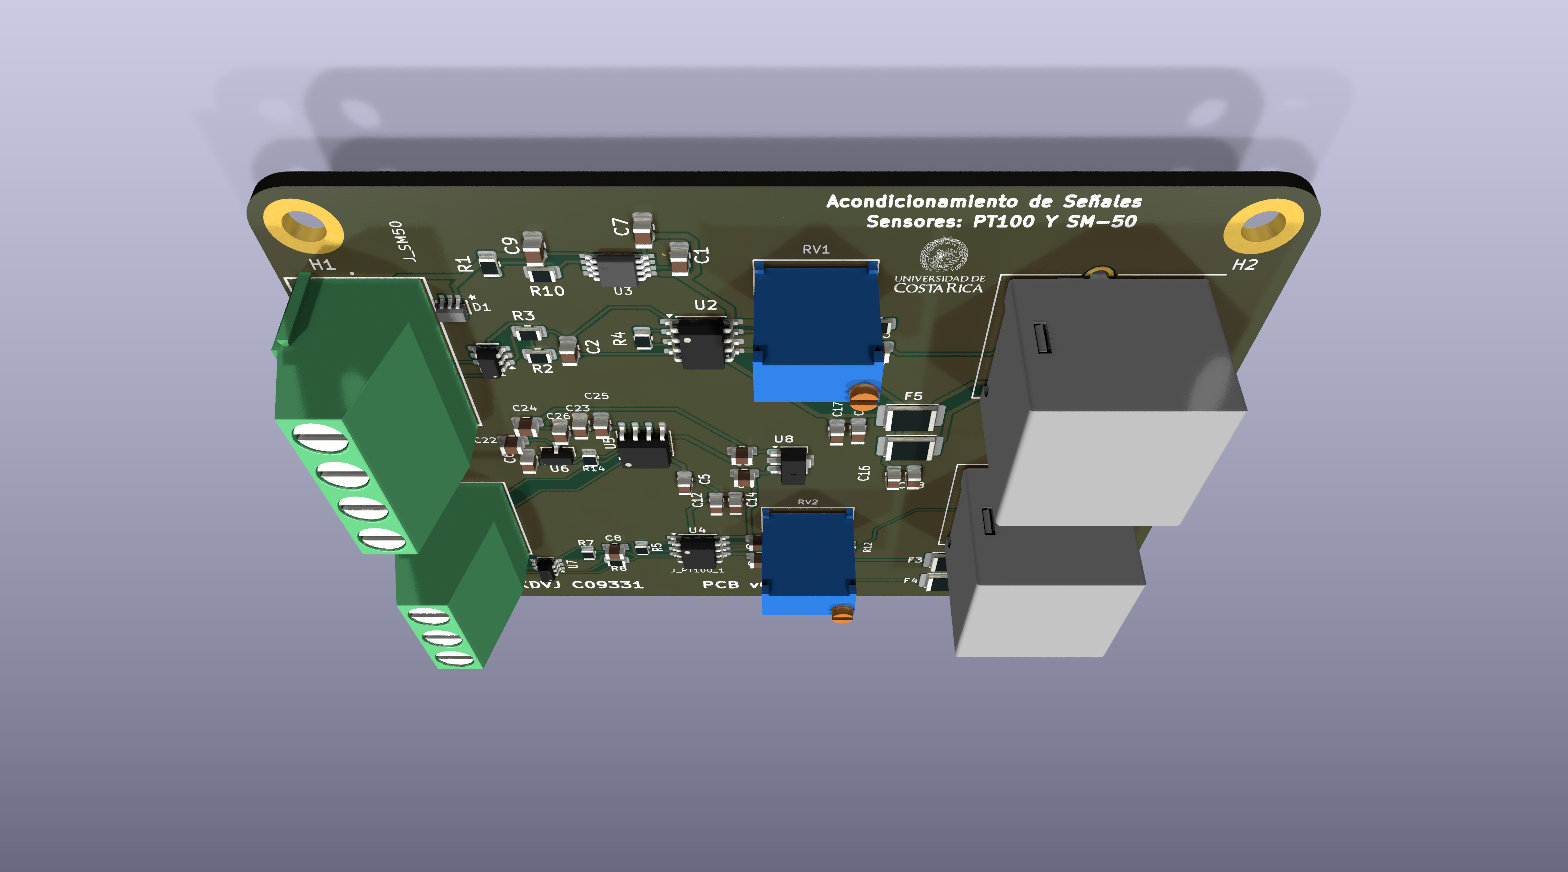
\includegraphics[width=0.82\textwidth]{kicad_pcb_3d.png}
\caption{Vista 3D de la PCB final en KiCad. La revisión permite verificar conectores, encapsulados y distribución física antes de fabricar.}
\label{fig:pcb}
\end{figure*}

\clearpage
\raggedbottom
\begin{thebibliography}{00}
\setlength{\itemsep}{0pt}
\setlength{\parsep}{0pt}
\bibitem{adi_paths} Analog Devices, ``Overview of Sensor Signal Paths,'' technical article, May 2010. [En línea]. Disponible: \url{https://www.analog.com/en/resources/technical-articles/overview-of-sensor-signal-paths.html}
\bibitem{adi_rtd} Analog Devices, ``How to Select and Design the Best RTD Temperature Sensing System,'' Analog Dialogue. [En línea]. Disponible: \url{https://www.analog.com/en/resources/analog-dialogue/articles/how-to-select-and-design-the-best-rtd-temperature-sensing-system.html}
\bibitem{ti_rtd} Texas Instruments, ``A Basic Guide to RTD Measurements,'' SBAA275A, application note, 2023. [En línea]. Disponible: \url{https://www.ti.com/lit/pdf/sbaa275}
\bibitem{bipm} BIPM, ``Guide on Secondary Thermometry: Industrial Platinum Resistance Thermometers,'' Consultative Committee for Thermometry, 2021. [En línea]. Disponible: \url{https://www.bipm.org/documents/20126/41773843/BIPM_CCT_Guide_to_IPRTs.pdf}
\bibitem{ina826} Texas Instruments, ``INA826 Precision, 200-uA Supply Current, 3-V to 36-V Instrumentation Amplifier,'' hoja de datos. [En línea]. Disponible: \url{https://www.ti.com/lit/ds/symlink/ina826.pdf}
\bibitem{ref30} Texas Instruments, ``REF30E and REF30 Low Current Voltage Reference in SOT-23-3,'' hoja de datos. [En línea]. Disponible: \url{https://www.ti.com/lit/gpn/REF30E}
\bibitem{opa2188} Texas Instruments, ``OPA2188 Low-Noise, 36-V, Zero-Drift Operational Amplifiers,'' hoja de datos. [En línea]. Disponible: \url{https://www.ti.com/lit/gpn/OPA2188}
\bibitem{tps7a49} Texas Instruments, ``TPS7A49 36-V, 150-mA, Ultralow-Noise Positive Linear Regulator,'' hoja de datos. [En línea]. Disponible: \url{https://www.ti.com/lit/gpn/TPS7A49}
\bibitem{interface} Interface Force Measurement Solutions, ``Model SM S-Type Load Cell,'' hoja de datos. [En línea]. Disponible: \url{https://www.scienspec.com.tw/userfiles/files/SM.pdf}
\bibitem{imperix} imperix, ``User Manual BoomBox,'' entradas analógicas y alimentación de sensores. [En línea]. Disponible: \url{https://imperix.com/wp-content/uploads/2018/06/User-Manual-BoomBox.pdf}
\bibitem{sloa034} Texas Instruments, ``Signal Conditioning Wheatstone Resistive Bridge Sensors,'' SLOA034. [En línea]. Disponible: \url{https://www.ti.com/lit/pdf/sloa034}
\bibitem{sboa247} Texas Instruments, ``Single-Supply Strain Gauge Bridge Amplifier Circuit,'' SBOA247A. [En línea]. Disponible: \url{https://www.ti.com/lit/pdf/sboa247}
\bibitem{an43} Analog Devices, ``AN-43: Bridge Circuits.'' [En línea]. Disponible: \url{https://www.analog.com/en/resources/app-notes/an-43f.html}
\bibitem{an96} Analog Devices, ``AN-96: Delta Sigma ADC Bridge Measurement Techniques.'' [En línea]. Disponible: \url{https://www.analog.com/en/resources/app-notes/an-96fa.html}
\bibitem{bourns3296} Bourns, ``3296 -- 3/8 Inch Square Trimpot Trimming Potentiometer,'' hoja de datos. [En línea]. Disponible: \url{https://www.bourns.com/docs/product-datasheets/3296.pdf}
\bibitem{bitacora} K. D. Vizcaíno Jiménez, ``Bitácora PCB PT100/SM-50 actualizada al 27 de junio de 2026,'' documentación interna del proceso de diseño, organización por ciudades, filtros, EMI y ruteo, 2026.
\bibitem{kicad_pcbnew} KiCad, ``PCB Editor Documentation: Board Setup, Design Rules, Net Classes and Track Width,'' documentación oficial, versión 8.0. [En línea]. Disponible: \url{https://docs.kicad.org/8.0/en/pcbnew/pcbnew.html}
\bibitem{digikey_trace} DigiKey, ``PCB Trace Width Conversion Calculator,'' herramienta técnica basada en IPC-2221. [En línea]. Disponible: \url{https://www.digikey.com/en/resources/conversion-calculators/conversion-calculator-pcb-trace-width}
\bibitem{cirexx_trace} Cirexx International, ``Trace Width Calculator,'' herramienta técnica basada en IPC-2221. [En línea]. Disponible: \url{https://www.cirexx.com/trace-width-calculator/}
\bibitem{labces_prev} LabCES, ``Caracterización de sensores y datos experimentales previos del banco de motor de inducción,'' documentación interna usada como antecedente experimental del proyecto, 2026.
\bibitem{repo} K. D. Vizcaíno Jiménez, ``Documentación interna del proyecto PCB PT100/SM50,'' cálculos, simulaciones, validación de diseño y paquete de fabricación, 2026.
\end{thebibliography}

\end{document}
